\documentclass[12pt, a4paper]{article}

\usepackage{amsmath}
\usepackage[utf8]{inputenc}
\usepackage[english]{babel}
% \usepackage[spanish]{babel} %Paquete de idioma
\usepackage[hidelinks]{hyperref}
\usepackage{graphicx}
\usepackage{float}
\usepackage{eso-pic}
\usepackage{lipsum}
\usepackage{transparent}
\usepackage{parskip}
%\usepackage[backend=biber, style=apa]{biblatex}

\graphicspath{{images_doc/}}

%%%%%%%%% ESTO PARA LA MARCA DE AGUA %%%%%%%%%%%%%%%%%%%%%%%%%%%%%%%


\AddToShipoutPicture{ 
    \put(470,370){
        \parbox[b][\paperheight]{\paperwidth}{%
            \vfill
            \
            {
            \transparent{1}
            
\includegraphics[scale=0.1]{uware_logo.png}
            % 
\includegraphics[scale=0.5]{logo-ua.png}
            \vfill
            }
        }
    }
}
%%%%%%%%%%%%%%%%%%%%%%%%%%%%%%%%%%%%%%%%%%%%%%%%%%%%%%%%%%

\title{Underwater pipe detector program   - Version 1} 


\author{
Leopoldo Cadavid Piñero
}








\begin{document}

\maketitle

\begin{figure}[H]
    \centering
    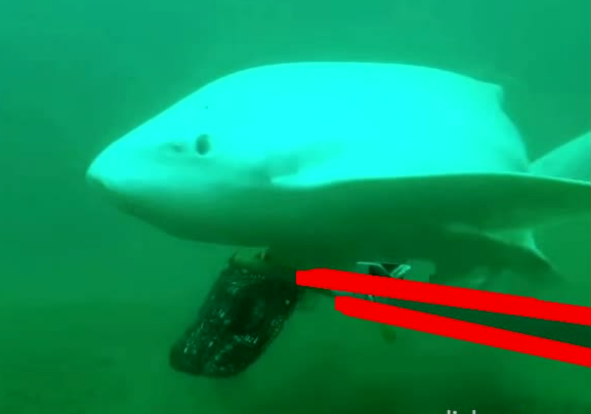
\includegraphics[scale=0.5]{images_doc/titel.png}
    
    \label{fig:repre}
\end{figure}

\newpage
\tableofcontents
\newpage

      
\section{Intro}

The main goal for this algorithm is to make possible human-made structures detection at underwater environments, making use of 
classic computer vision techniques.

Especifically, this first version of the algorithm is focused on pipes or similar structures. 

\section{Preprocessing}\label{ch:preprocesamiento}

First of all, is necessary to apply some preprocessing methods to get our images 
\textit{cleaner} before trying to get features from them. Preprocessing pipeline 
consist on 2 parts:

\begin{itemize}
    
    \item Apply a mask in order to increase contrast, decreasing L value in CIELAB channel space in our picture.
    This is done because we want to
    compensate colour distorsion result from ligth propagation along the picture. 
        

    \item Second, we use a CLAHE ( \textit{contrast-limited adaptive histogram equalization} ) in order to 
    \textbf{redistribute luminescence}.
    
    

\end{itemize}

La aplicación de los métodos da como resultado una imagen mán nítida y contrastada
 donde es más fácil aplicar los algoritmos para la segmentación y detección de las estructuras.


\section{Image Processing}

\subsection{First approach: K-means algorithm}


Based on referenced papers, the use of Sobel filter to get gradient response on different directions. Then 
this response would be used to create a \textbf{features vector}. The final step would be to classiffy objects 
using K-means algorithm with this feature array as entrance. 

% \textbf{Primeros resultados:} tras aplicar el método descrito, las clusterización no arroja una segmentación prometedora.
% Los fallos posibles:
% \begin{itemize}
%     \item Que los bordes no sean una características significativa a la hora de detectar
%     el objeto. 

%     \item Una implementación errónea del algoritmo a partir de la descripción. 
%     \item Una representación errónea de los datos.
% \end{itemize}

At a first stage in the studies of the algorithm, no significative resutls were provided by this methon. 

However, due to no progression on our second approach, it was decided to retake K-means idea. 

Currently, big advances have been made, as it has been correctly implmenetated in a python script. In summary, 
the methodology has been the following: 

\begin{itemize}
    \item Apply CLAHE + blur L channel for improving quality in our image.
    \item Apply white balancing in order to achieve a more accurate color space (based on Gray world theory)
    \item Apply Sobel filtering to each hsv channel, for achiving gradients on each channel
    \item Create a features vector, each pixel has the following features: \textbf{F(H, S, V, GradR, GradG, GradB)}
    \item Apply k-means algorithm to our features vector, so we are getting N clusters of pixels. 
    \item Reagrupate our clusters and process information. (this is described on image post processing section)
\end{itemize}

Above, in section \ref{ch:results} more specific details of our algorithm results will be explained. Some of the clusters 
detected are the following. 


\subsection{Second approach: detection based on lines}\label{ch:second_approach}



In this case, based on certain ideas discussed in the previous approximation,
we're trying get a different pipeline from the studied one.  The steps followed
in this case they have been the following:

\begin{itemize}
    
    \item Perform preprocessing, as described in \Ref{ch:preprocesamiento}.
    
    \begin{figure}[H]
        \centering
        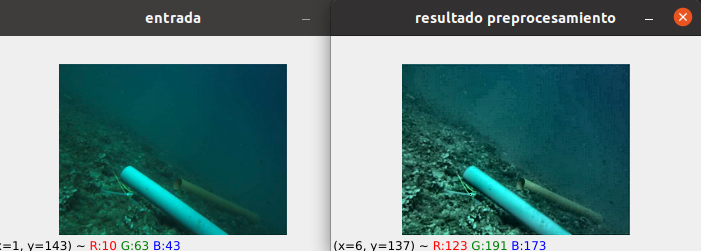
\includegraphics[scale=0.3]{images_doc/preprocess.png}
        \caption{Before-After preprocessing}
        \label{fig:pprepre}
    \end{figure}

    \item Apply a bilateral filter to remove some background noise from images.
    
    \begin{figure}[H]
        \centering
        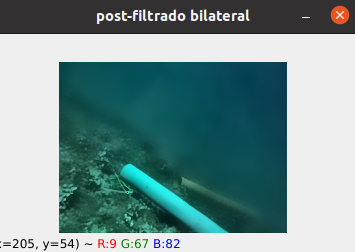
\includegraphics[scale=0.3]{images_doc/filtradobilat.png}
        \caption{bilateral filter}
        \label{fig:bilat}
    \end{figure}

    \item Apply \verb|PyrMeanShift()|, so that the image is segmented by colors.
    
    \begin{figure}[H]
        \centering
        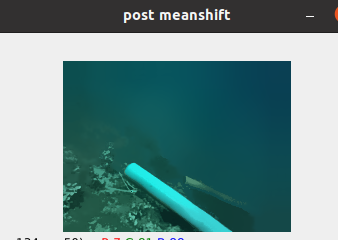
\includegraphics[scale=0.3]{images_doc/meanshift.png}
        \caption{Meanshift segmentation}
        \label{fig:menas}
    \end{figure}

    \item Apply the algorithm \textbf{Sobel()}, to each of the channels of thepreprocessed  image
    RGB. This is done to get the gradient changes and is applied equally
    to the X and Y axes, performing a weighted sum of both in order to obtain the
    change in different directions.

    \begin{figure}[H]
        \centering
        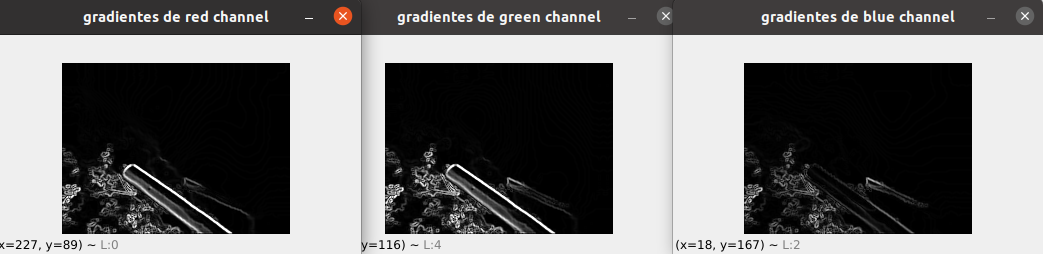
\includegraphics[scale=0.3]{images_doc/gradientes.png}
        \caption{Sobel gradients splitted}
        \label{fig:Sobel}
    \end{figure}

    \item Obtain, from the gradients, edges in the images applying the
    algorithm \verb|Canny()|.

    \begin{figure}[H]
        \centering
        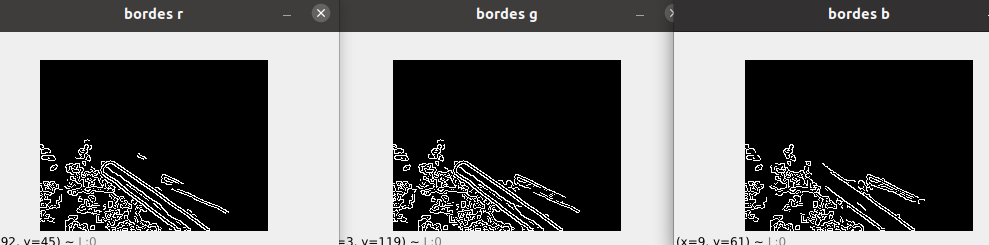
\includegraphics[scale=0.3]{images_doc/bordes.png}
        \caption{Edges with Canny}
        \label{fig:Canny}
    \end{figure}


    \item We use morphological filters to erode and dilate, trying to eliminate,
    circular elements that may disturb and then we amplify rectangular elements.

    \begin{figure}[H]
        \centering
        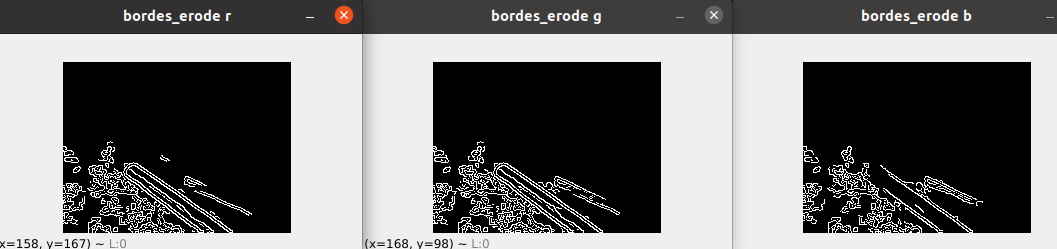
\includegraphics[scale=0.3]{images_doc/bordes_erode.png}
        \caption{Edges after morphological transformations}
        \label{fig:erodes}
    \end{figure}



    \item Having the edges filtered, the Hough transform is used to find lines in
    inside the image.

    \begin{figure}[H]
        \centering
        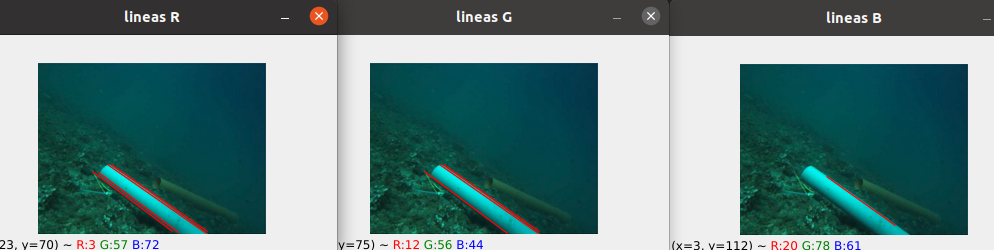
\includegraphics[scale=0.3]{images_doc/lineas_separada.png}
        \caption{Lines from Hough transform}
        \label{fig:jiug}
    \end{figure}
    
    \item From the 3 line vectors we have, we create a new one where we will join
    \textbf{all lines in the image}.
    
\end{itemize}

% \begin{figure}[H]
%     \centering
%     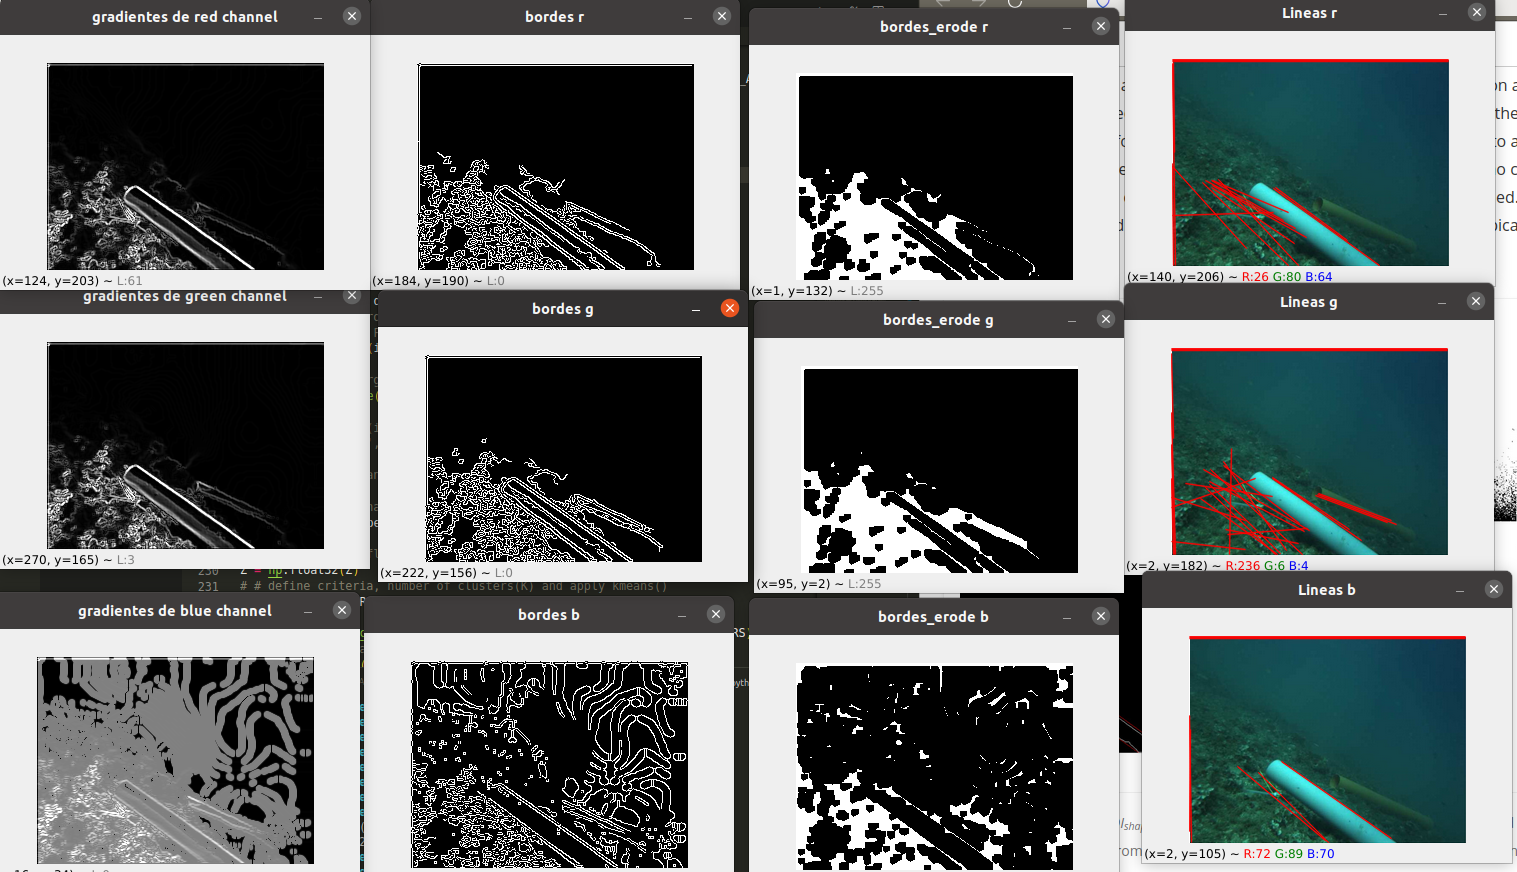
\includegraphics[scale=0.3]{sobel_canny_houghlines.png}
%     \caption{Lines obtained for each channel in one of the images studied}
%     \label{fig:sobelcanny}
% \end{figure}
\begin{figure}[H]
    \centering
    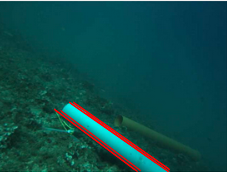
\includegraphics[scale=0.3]{images_doc/all_lines.png}
    \caption{Lines from Hough transform}
    \label{fig:jiiug}
\end{figure}

\section{Post Processing}

\subsection{Cluster management}

After obtaning the clusters from the image, its necessary to get the mask from this
information. 

\subsection{Line filtering}


From the extracted lines, it seeks to dete lines that do not correspond to those belonging to the real pipe. For this, it will be analyzed
both the degree of parallelism and the distance between them.

The idea is to analyze in the vector of lines each pair of these in the following way:


\begin{itemize}

    \item The slope and the angle of each of these with respect to the front are calculated
    \item The angles are compared and, if they are below a certain threshold, the lines will be considered parallel
    \item The distances in X and Y of the initial points of each line are compared, and we are left with those that are below
    a threshold away
    \item Lines that meet all conditions will be saved in a vector of parallel lines
\end{itemize}

\textbf{Update:} One of the updates implemented has been a new algorithm for parallel lines. 
First algorithm worked well when recognising parallelism between any kind of lines, 
desafortunatedly, it was a problem when many noise lines appear, because it turns out in 
many parallel non-significative lines.

Because of this, another criteria was tried. I could notice that, in most of the cases, 
the biggest line founded was always on our pipe so, instead of studying parallelism between all
pairs of lines, you could only compare lines with the bigger one , this wouls help eliminating problems
with noisy lines. The biggest issue with this new algorithm is that it relays on the assumption that the 
biggest line will be alway on the path.

After filtering the lines, these are highlighted on the original image, applying certain morphological filters to improve their shape, and we finally obtain the
image with the mask applied on the structure.

\section{Subsection}



\subsection{Used Dataset}

Before showing the results, the images and video used to study the operation of the algorithm will be shown:

\begin{figure}[H]
    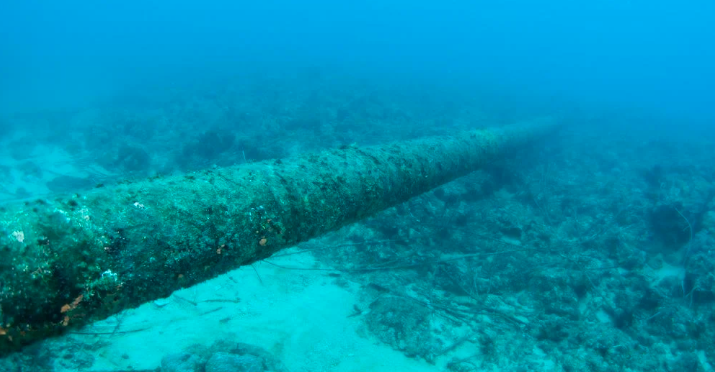
\includegraphics[width=.24\textwidth]{images_doc/img1.png}\hfill
    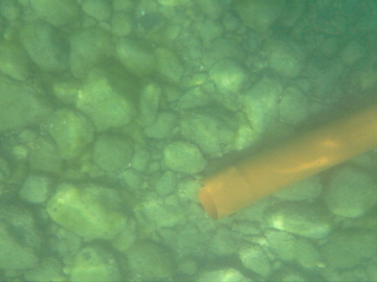
\includegraphics[width=.24\textwidth]{images_doc/img2.png}\hfill
    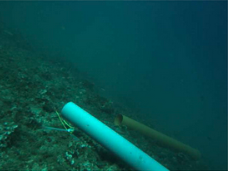
\includegraphics[width=.24\textwidth]{images_doc/img3.png}\hfill
    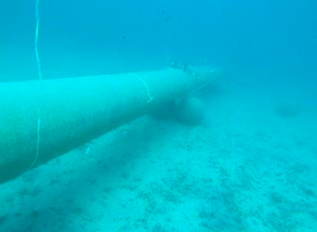
\includegraphics[width=.24\textwidth]{images_doc/img4.png}
    \\[\smallskipamount]
    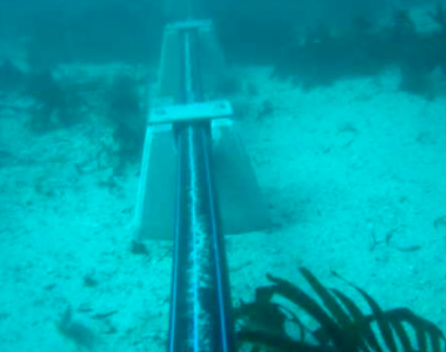
\includegraphics[width=.24\textwidth]{images_doc/img5.png}\hfill
    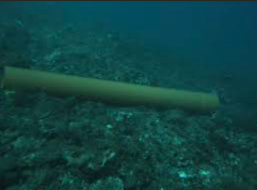
\includegraphics[width=.24\textwidth]{images_doc/img6.png}\hfill
    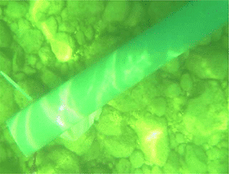
\includegraphics[width=.24\textwidth]{images_doc/img7.png}\hfill
    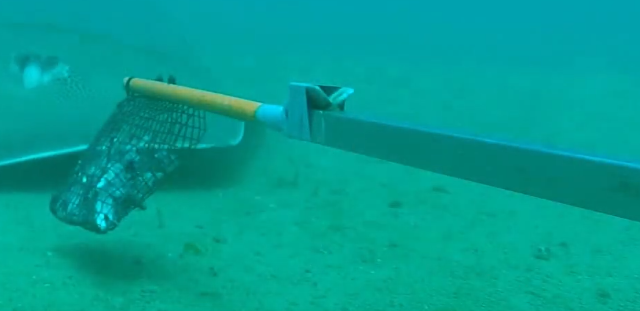
\includegraphics[width=.24\textwidth]{images_doc/img8.png}
   
    \caption{Some images}\label{fig:foobar}
\end{figure}

This youtube video has been used for video detection: \href{https://youtu.be/L0Ev5R3fBEc}{https://youtu.be/L0Ev5R3fBEc}

% \newpage
% \begin{figure}[H]
%     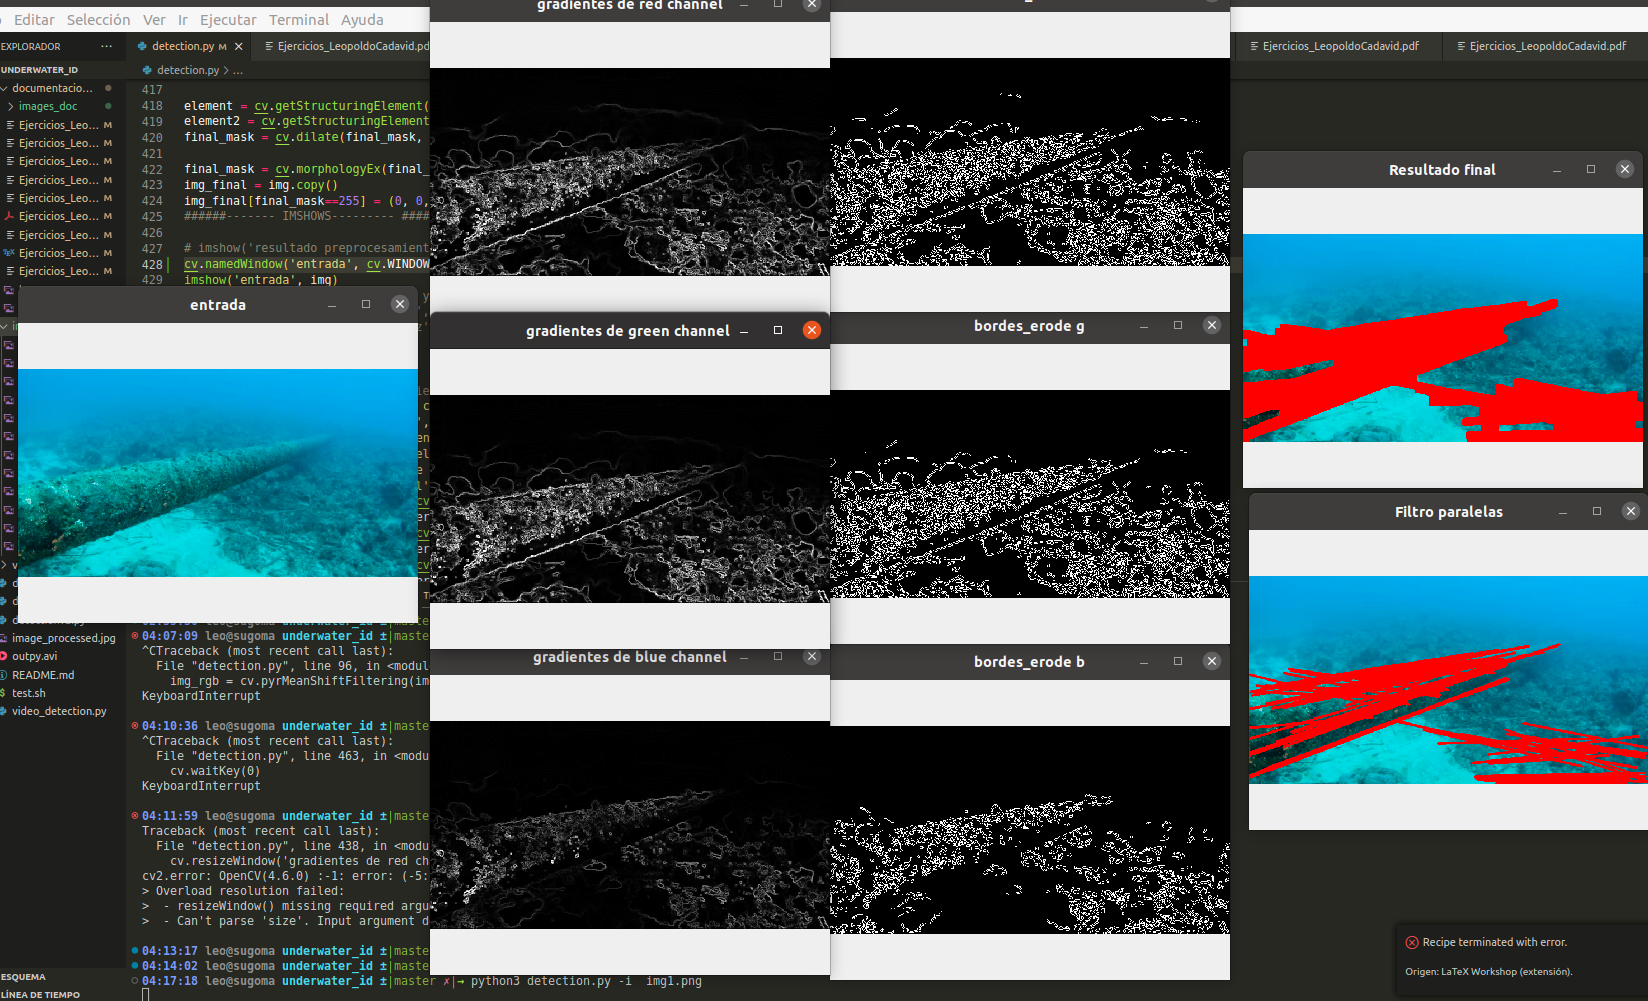
\includegraphics[scale=0.22]{images_doc/img1_results.png}
%     \caption{res1}\label{fig:im1r}
% \end{figure}

% \newpage
% \begin{figure}[H]
%     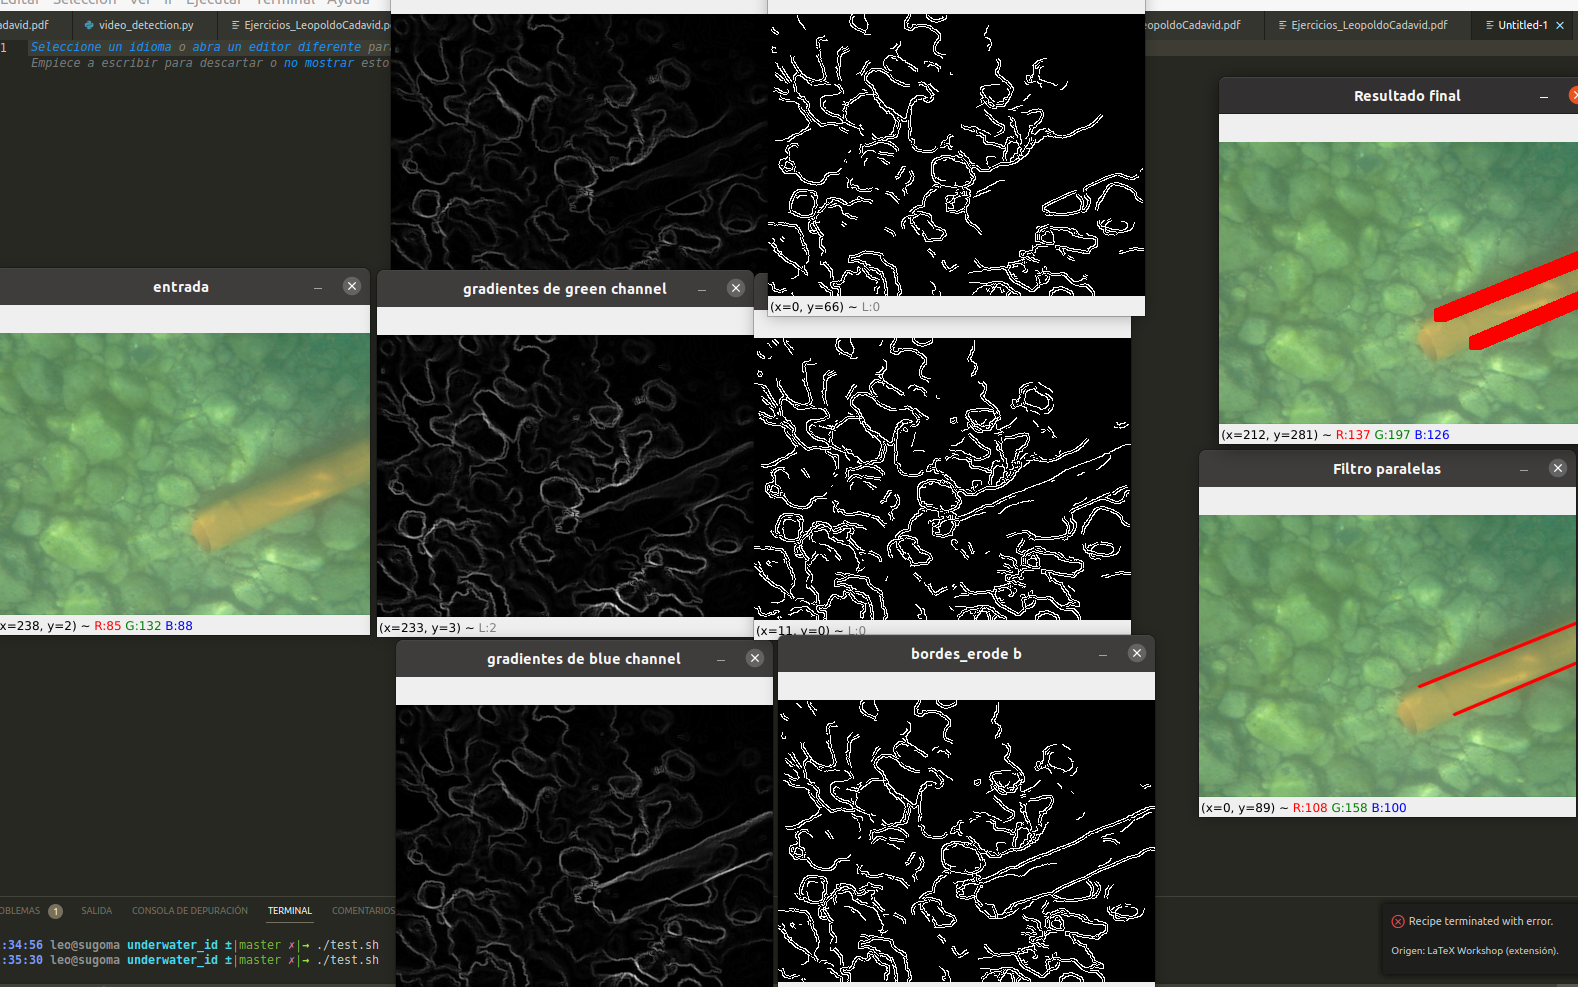
\includegraphics[scale=0.22]{images_doc/img2_results.png}
%     \caption{res1}\label{fig:im2r}
% \end{figure}
% \newpage
% \begin{figure}[H]
%     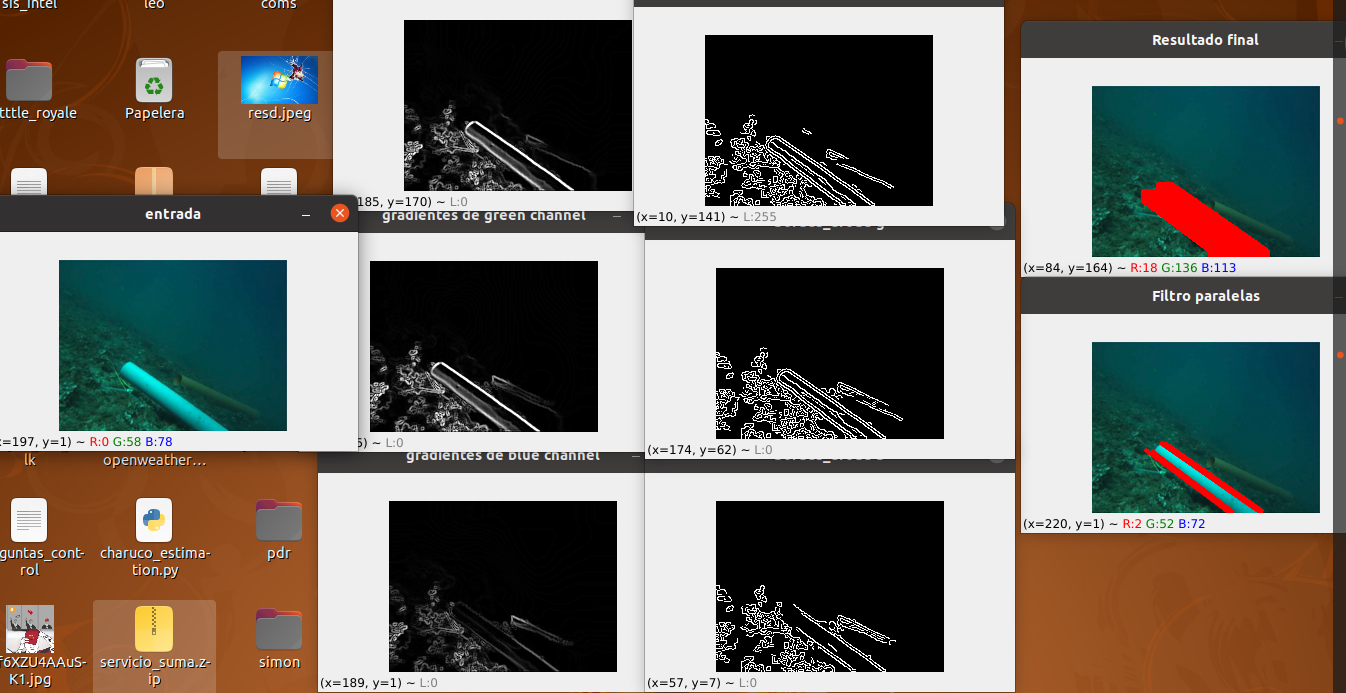
\includegraphics[scale=0.22]{images_doc/img3_results.png}
%     \caption{res1}\label{fig:im3r}
% \end{figure}

% \newpage
% \begin{figure}[H]
%     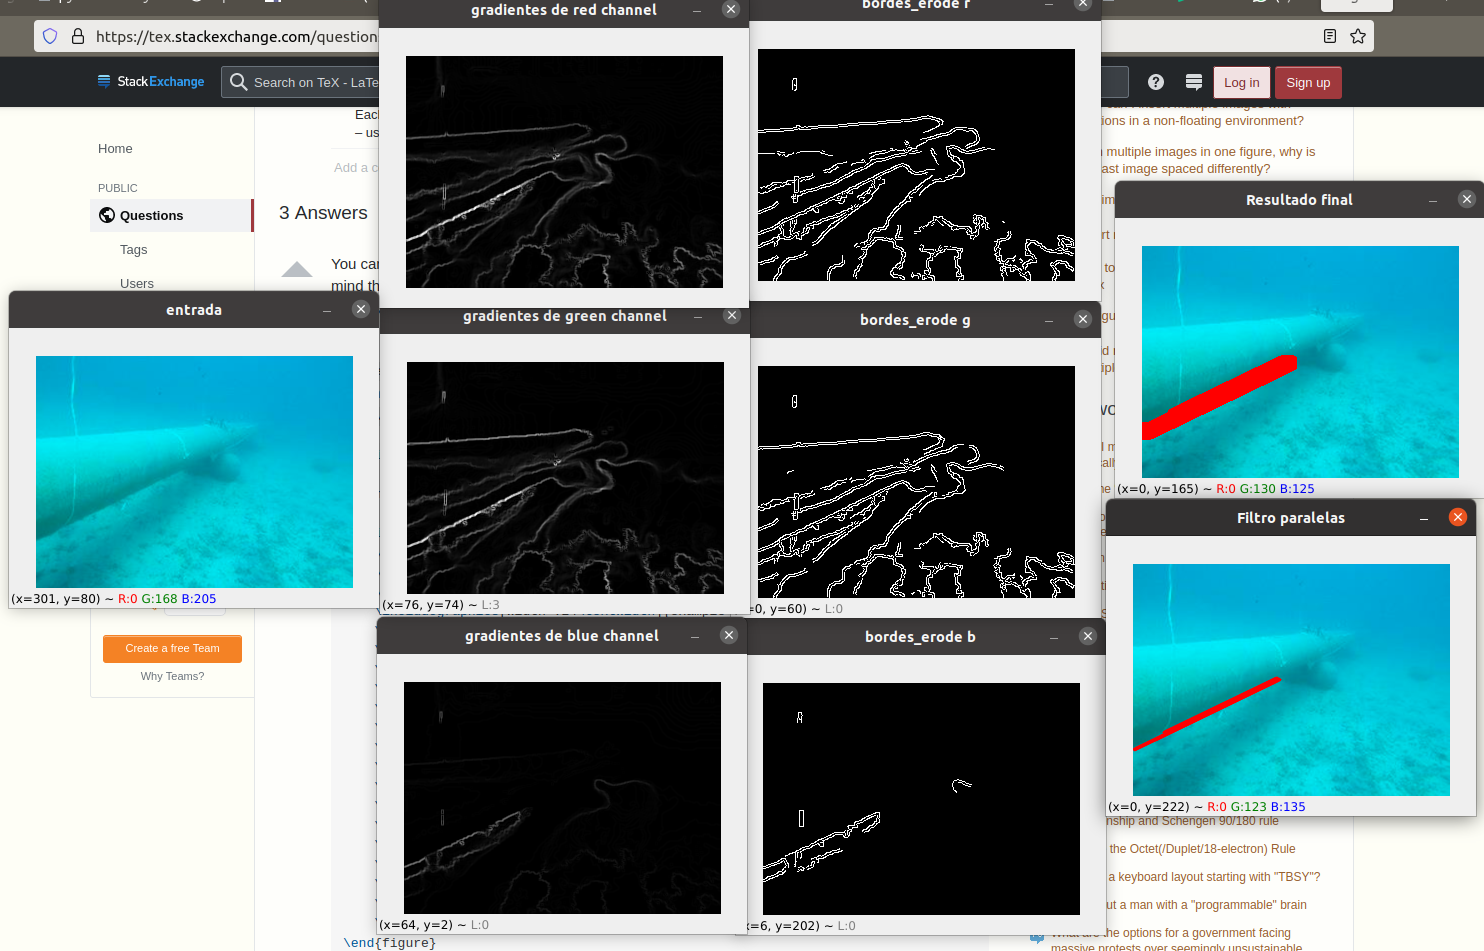
\includegraphics[scale=0.22]{images_doc/img4_results.png}
%     \caption{res1}\label{fig:im4r}
% \end{figure}
% \begin{figure}[H]
%     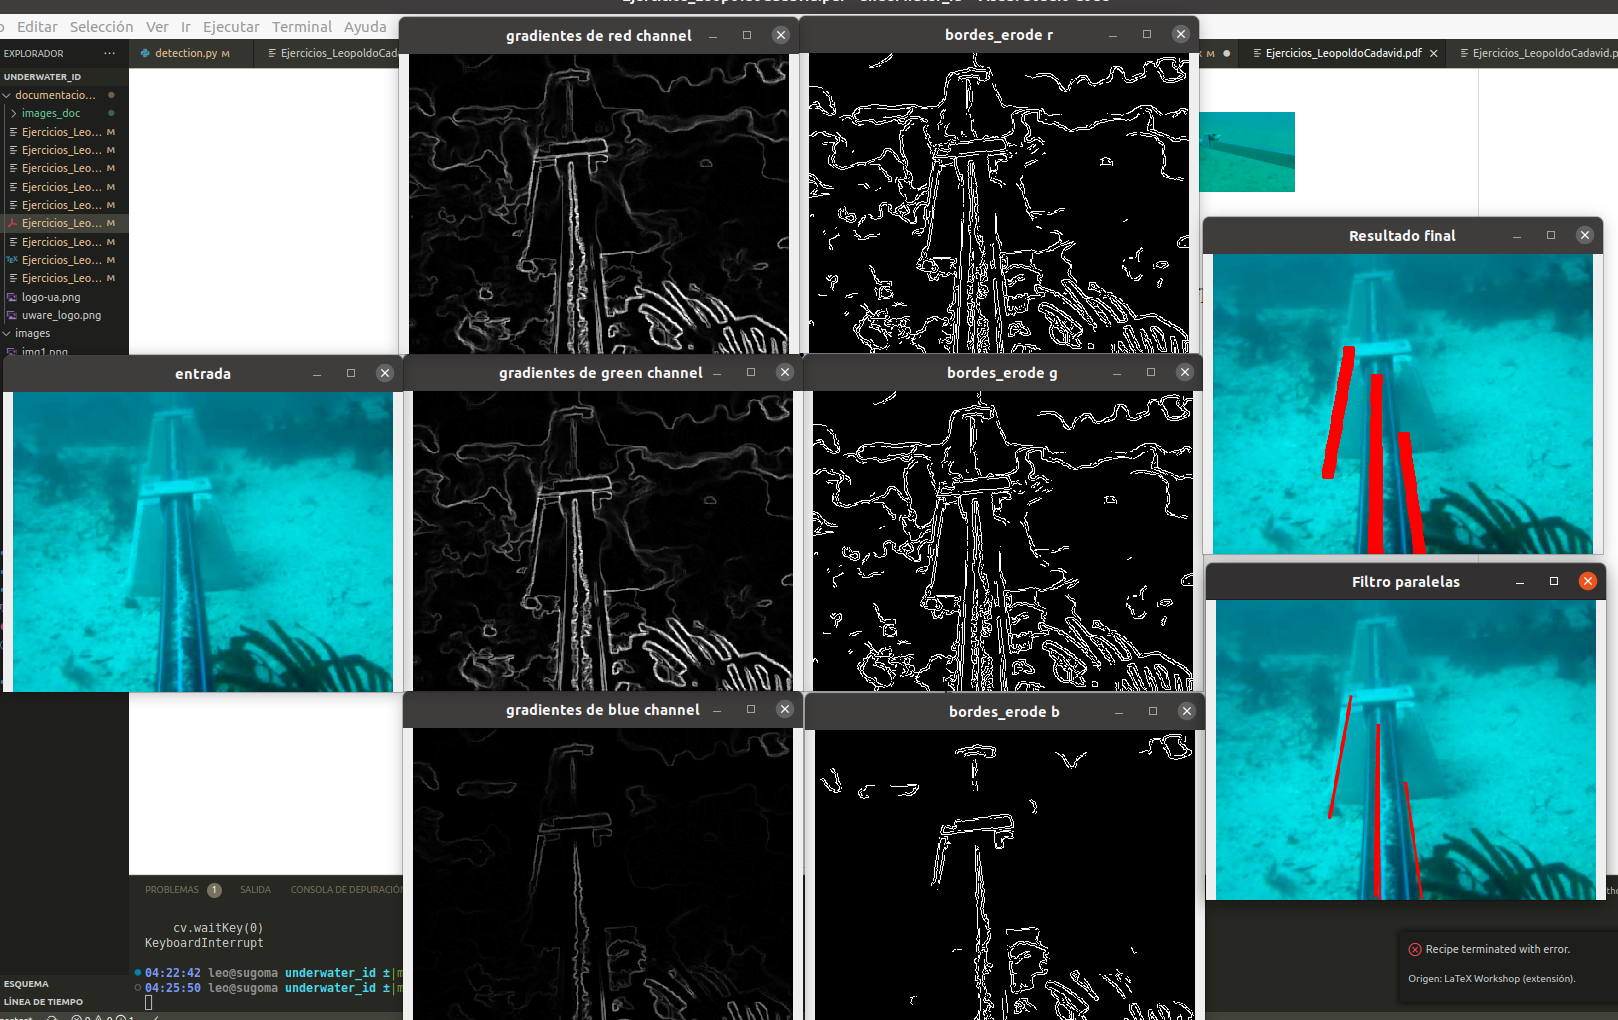
\includegraphics[scale=0.22]{images_doc/img5_results.png}
%     \caption{res1}\label{fig:im5r}
% \end{figure}

% \newpage
% \begin{figure}[H]
%     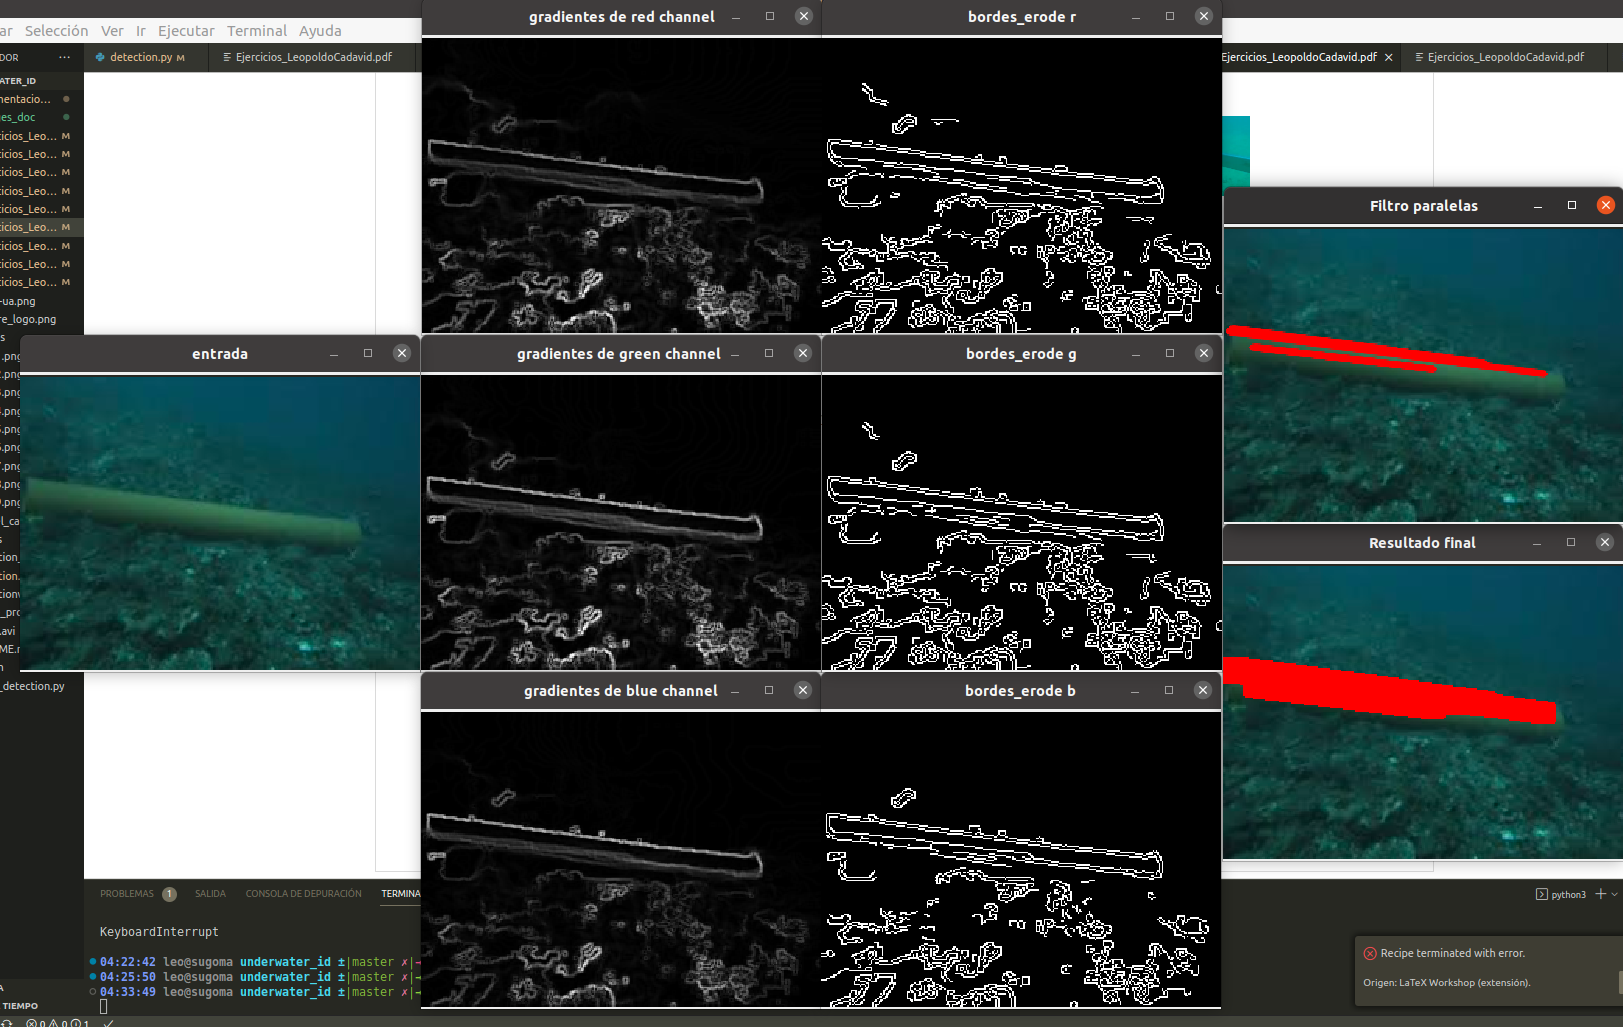
\includegraphics[scale=0.22]{images_doc/img6_results.png}
%     \caption{res1}\label{fig:im6r}
% \end{figure}
% \newpage
% \begin{figure}[H]
%     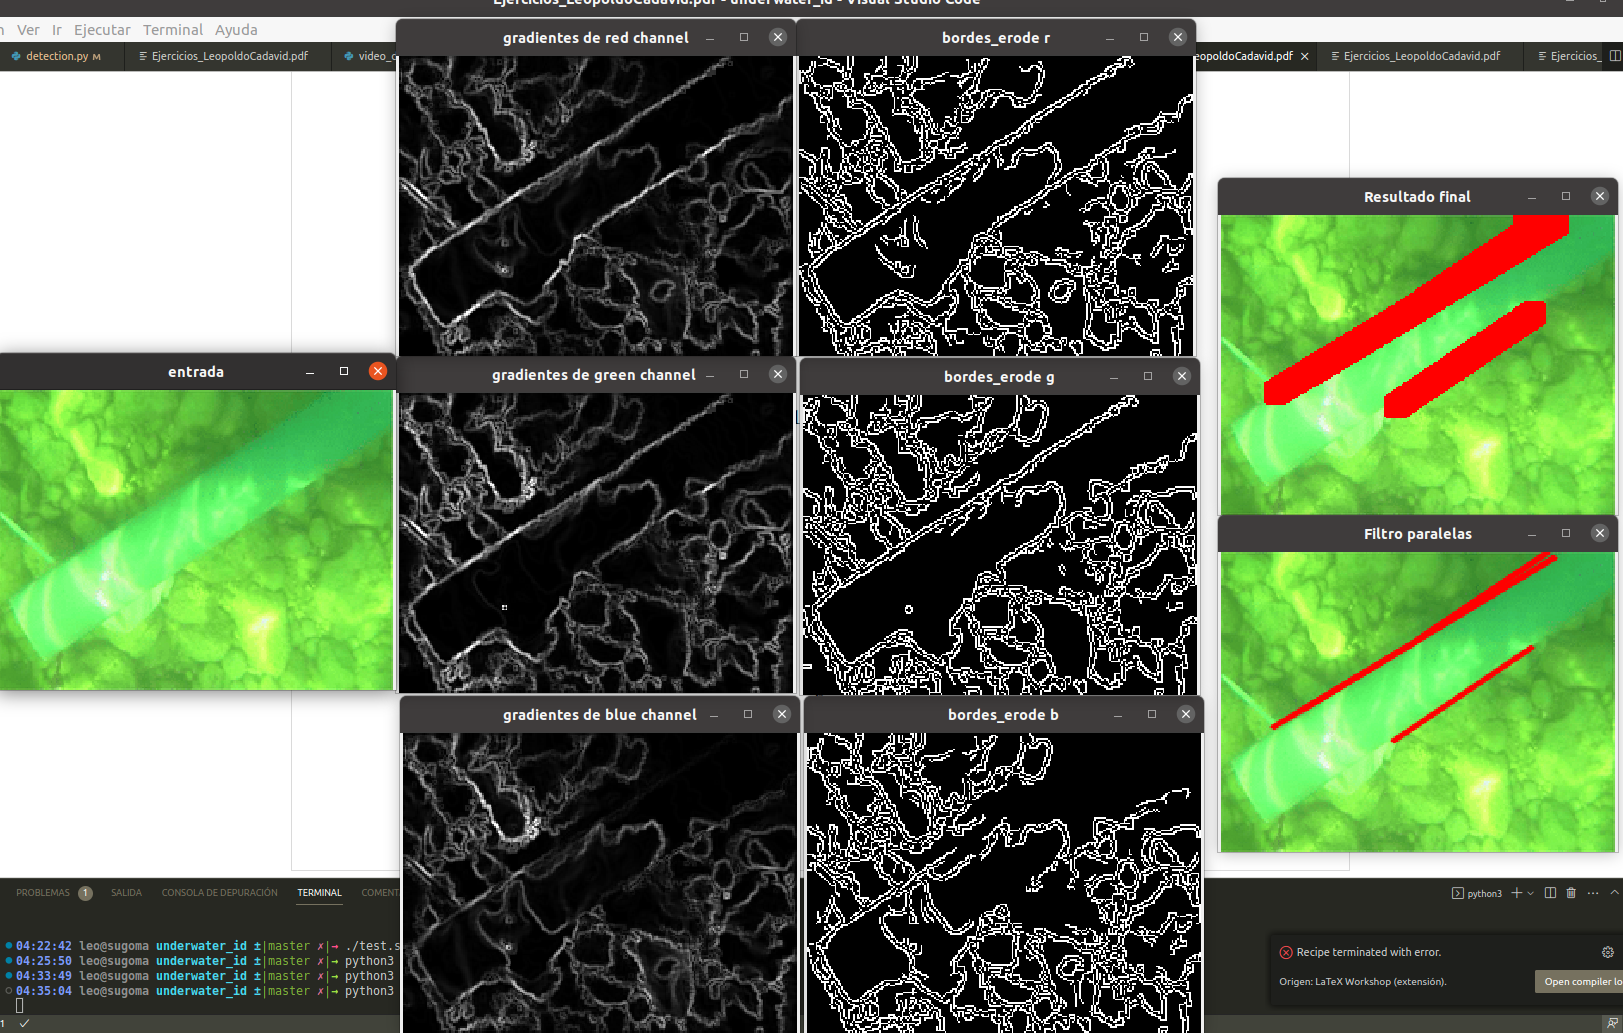
\includegraphics[scale=0.22]{images_doc/img7_results.png}
%     \caption{res1}\label{fig:im7r}
% \end{figure}

% \newpage
% \begin{figure}[H]
%     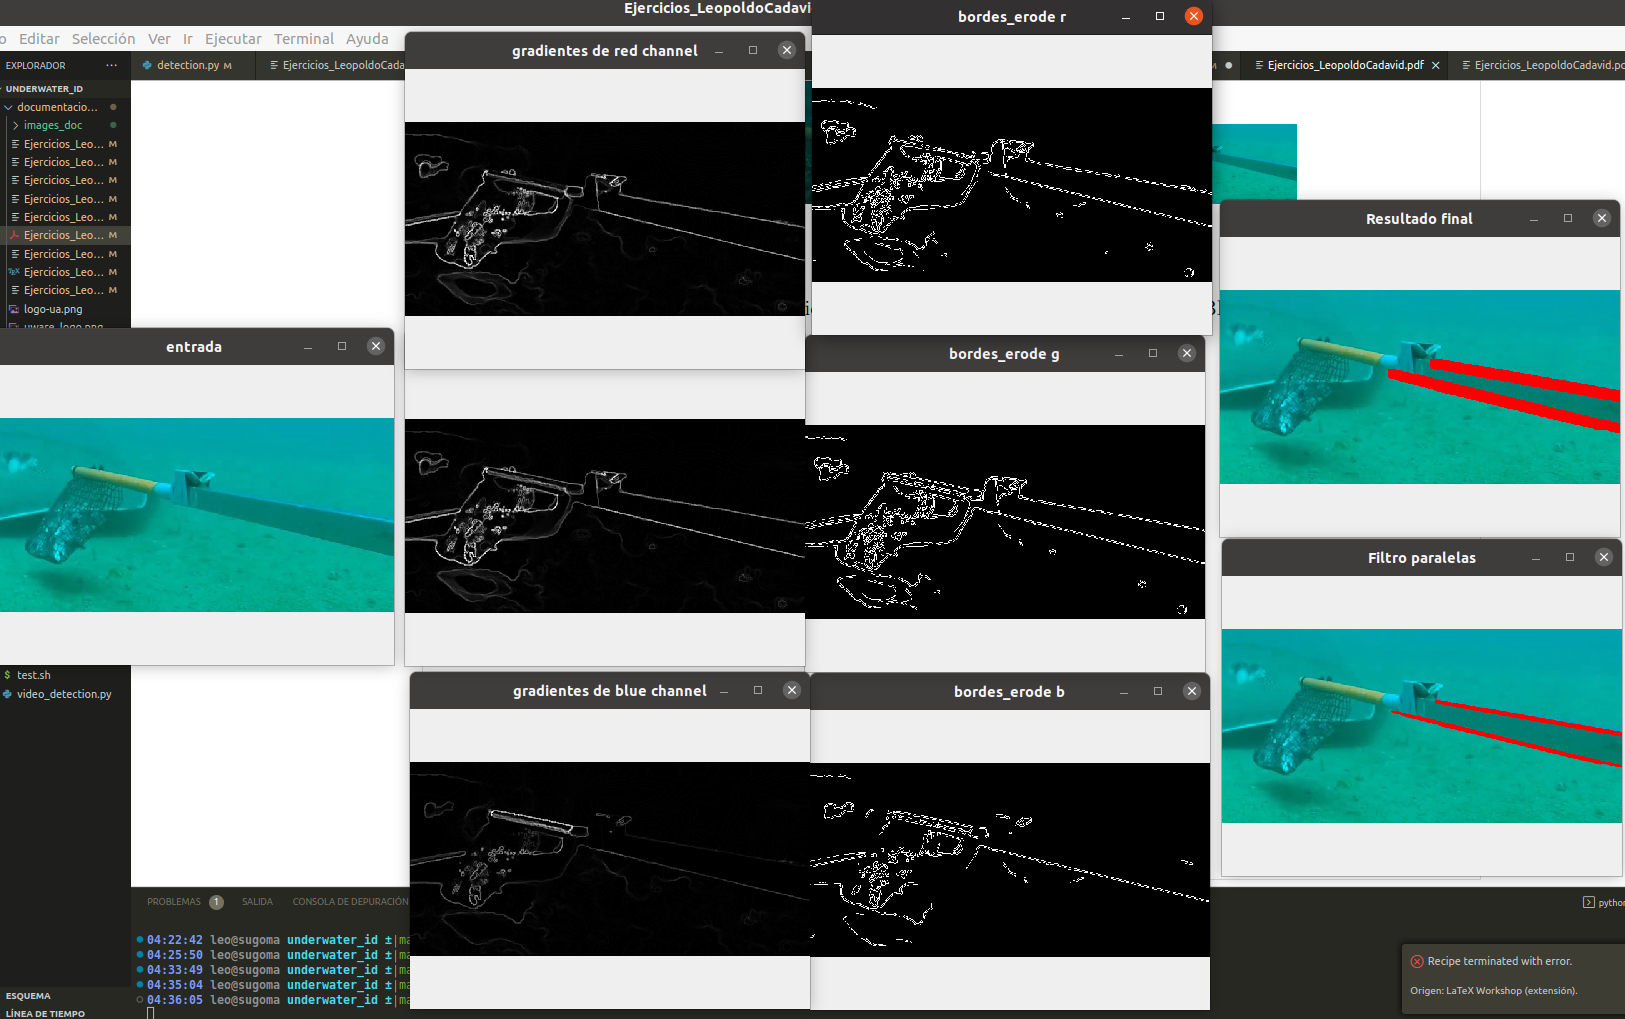
\includegraphics[scale=0.22]{images_doc/img8_results.png}
%     \caption{res1}\label{fig:im8r}
% \end{figure}

% \subsection{Possible improvements}





\section{Performed tests}

\subsection{Methrics and testing methodology}

There have been 2 different kind of tests applied to each pipeline, accuracy and time-performance tests. 

For each one, we are going to explain which methrics have been used: 

\begin{itemize}
    \item \textbf{Intersection of Unions:} is a way to measure the similarity between two sets of data. 
    To calculate this metric, we first take the union of both sets, 
    which represents all the elements that are present in either set. 
    We then take the intersection of the two sets, which represents the elements that 
    are common to both sets. The intersection of unions metric is 
    then calculated by dividing the size of the intersection by the size of the union. 


    \item \textbf{Execution time in miliseconds:} provided by \textit{Time} library in Python. 
\end{itemize}

Going deep inside testing methodology, for our accuracy tests, what has been done is the next: 

\begin{itemize}
    \item Paint, manually, an ideal mask on each image of our dataset.
    \item Calculate intersection of unions for each image, betweem 
    the mask produced by our algorithm and the ideal mask. 
    \item Show each accuracy one by one and, finally, a mean accuracy in our algorithm. 
\end{itemize}


On the other hand, when testing time performance, what has been done is the following: 

\begin{itemize}
    \item Split the code in separated functions, each one corresponding to one of the processes in our
        pipeline. 
    \item Take the execution moment at the beggining and in the end of every function. The difference between
    this moments corresponds with the time execution taken by the process. 
\end{itemize}

\section{Results}

\subsection{K-means approach}

\subsection{Lines approach}




\subsection{Change PyrMeanShift parameters}

As was described in section \ref{ch:second_approach}, \verb|PyrMeanShift()| algorithm
is used for decreasing noise after preprocessing our image. Specifically, its
aim is to do colout segmentation based on 2 types of neighborhoodness: by colour
and by space. 

Testing this function, the parameters that have been tuned are the following 
ones: 

\begin{itemize}
    
    \item  Spacial neighborhood radius was increased. This would help the algorithm
    find more same-colour pixels in a bigger range. 
    
    \item Colour neighborhood radius was decreased. Because of this, less pixels 
    will be considered as \textit{same-coloured}. This produces a smaller segmentations.

    \item Max level of segementation has been elevated, meaning that we will get 
    less contours as segmentation has been bigger.

\end{itemize}


This test have shown that, scalating coulour neighborhood can reduce noise significatively 
but, as a takeoff, it can erase part of our structure, destying performance.


% \section{findparallel2()}

% One of the actualizatons implemented has been a new algorithm for parallel lines. 
% First algorithm worked well when recognising parallelism between any kind of lines, 
% desafortunatedly, it was a problem when many noise lines appear, because it turns out in 
% many parallel non-significative lines.

% Because of this, another criteria was tried. I could notice that, in most of the cases, 
% the biggest line founded was always on our pipe so, instead of studying parallelism between all
% pairs of lines, you could only compare lines with the bigger one , this wouls help eliminating problems
% with noisy lines. The biggest issue with this new algorithm is that it relays on the assumption that the 
% biggest line will be alway on the path.

\section{Results}\label{ch:results}

\section{Referencias}

https://journals.sagepub.com/doi/10.5772/60526
http://www.ce.unipr.it/~rizzini/papers/kallasi15oceans.pdf
% \begin{figure}[H]
%     \centering
%     \includegraphics[scale=0.1]{tarea_1roscore.png}
%     \caption{Lanzamos el master}
%     \label{fig:tarea1roscore}
% \end{figure}



\end{document}